% =====================================================================
%  HATI explained. A plain-language guide to the plots and the numbers.
%  Author: Gergő Csaba Morvai
%  Engine: LuaLaTeX  (compile: latexmk -lualatex hati_explained.tex)
% =====================================================================
\documentclass[11pt]{article}

\usepackage{fontspec}
\usepackage{microtype}
\usepackage[a4paper,margin=2.4cm]{geometry}
\usepackage{graphicx}
\graphicspath{{../output/athena/}{../dashboard/static/assets/}{../output/}}
\usepackage{amsmath,amssymb}
\usepackage{xcolor}
\usepackage{booktabs}
\usepackage{array}
\usepackage{siunitx}
\usepackage[font=small]{caption}
\usepackage{enumitem}
\usepackage{tcolorbox}
\tcbuselibrary{skins,breakable}
\usepackage{titlesec}
\usepackage[backend=biber,style=authoryear,sorting=nyt,maxcitenames=2,uniquelist=false]{biblatex}
\addbibresource{references.bib}
\usepackage[hidelinks]{hyperref}
\usepackage{cleveref}

\setmainfont{TeX Gyre Pagella}
\setsansfont{TeX Gyre Heros}[Scale=0.92]
\setmonofont{TeX Gyre Cursor}[Scale=0.90]

% ---- HATI brand palette ----
\definecolor{hatinavy}{HTML}{0D1B2A}
\definecolor{hatiblue}{HTML}{1F3A5F}
\definecolor{hatired}{HTML}{C1121F}
\definecolor{hatisilver}{HTML}{8B97A5}
\definecolor{hatiteal}{HTML}{1B7A6E}
\definecolor{plainbg}{HTML}{EAF2FB}
\definecolor{keepbg}{HTML}{EAF5EF}
\definecolor{limitbg}{HTML}{FBEEEC}

\titleformat{\section}{\sffamily\Large\bfseries\color{hatinavy}}{\thesection}{0.6em}{}
\titleformat{\subsection}{\sffamily\large\bfseries\color{hatiblue}}{\thesubsection}{0.5em}{}
\titlespacing*{\section}{0pt}{1.7ex plus .3ex}{0.8ex}

\newtcolorbox{plainbox}[1][In plain words]{breakable,enhanced,colback=plainbg,
  colframe=hatiblue,boxrule=0.6pt,arc=2pt,left=7pt,right=7pt,top=4pt,bottom=4pt,
  fonttitle=\bfseries\sffamily\small,coltitle=hatiblue,
  attach boxed title to top left={xshift=8pt,yshift=-7pt},
  boxed title style={colback=plainbg,colframe=hatiblue,boxrule=0.4pt,arc=1pt},title={#1}}
\newtcolorbox{keepbox}[1][What this tells us]{breakable,enhanced,colback=keepbg,
  colframe=hatiteal,boxrule=0.6pt,arc=2pt,left=7pt,right=7pt,top=4pt,bottom=4pt,
  fonttitle=\bfseries\sffamily\small,coltitle=hatiteal,
  attach boxed title to top left={xshift=8pt,yshift=-7pt},
  boxed title style={colback=keepbg,colframe=hatiteal,boxrule=0.4pt,arc=1pt},title={#1}}
\newtcolorbox{limitbox}[1][Honest limit]{breakable,enhanced,colback=limitbg,
  colframe=hatired,boxrule=0.6pt,arc=2pt,left=7pt,right=7pt,top=4pt,bottom=4pt,
  fonttitle=\bfseries\sffamily\small,coltitle=hatired,
  attach boxed title to top left={xshift=8pt,yshift=-7pt},
  boxed title style={colback=limitbg,colframe=hatired,boxrule=0.4pt,arc=1pt},title={#1}}

\sisetup{detect-all,per-mode=symbol}
\DeclareSIUnit{\px}{px}
\setlist{nosep,leftmargin=1.4em}
\captionsetup{labelfont={bf,sf,color=hatinavy}}
\pagestyle{plain}

\begin{document}

% ---------------------------------------------------------------- cover
\begin{titlepage}
\centering
\vspace*{2.2cm}

\includegraphics[width=6.2cm]{hati_logo.png}\\[1.4cm]
{\sffamily\bfseries\fontsize{27}{31}\selectfont\color{hatinavy}
Finding the hazards a map cannot see}\\[10pt]
{\sffamily\Large\color{hatiblue} A plain-language guide to HATI:\\ what it measures, what the plots show,
and what the numbers mean}\\[1.6cm]
{\color{hatired}\rule{9cm}{1.2pt}}\\[1.1cm]
{\large Gergő Csaba Morvai}\\[4pt]
{\normalsize\itshape M\'ani Mission terrain-hazard pipeline}\\[4pt]
{\normalsize June 2026}
\vfill
{\footnotesize\color{hatisilver}\sffamily
HAZARD ASSESSMENT AND TERRAIN INTELLIGENCE}
\end{titlepage}

% ---------------------------------------------------------------- intro
\section{What this document is}

This is the guide for anyone who wants to understand HATI without a background in
planetary science. It walks through each figure the project produces, says what you
are looking at, and explains what every number means and why it matters. No prior
knowledge is assumed. Technical terms are defined the first time they appear and
again in the glossary at the back.

The short version: HATI looks at pictures and elevation maps of the Moon taken from
orbit, and tries to work out which patches of ground would be dangerous to land on.
The interesting part is that the most dangerous things are usually too small for the
maps to show, so HATI has to find them indirectly.

% ---------------------------------------------------------------- why
\section{Why this exists}

On 6 March 2025 a spacecraft called IM-2, nicknamed Athena, landed near the Moon's
south pole and tipped over. Analysis afterwards pointed to a crater about
\SI{20}{\meter} across on gently sloped ground, right where it set down.

That is the whole problem in one sentence. The elevation maps used to choose the
landing site had a resolution of about \SI{4}{\meter} per pixel, and in practice they
cannot resolve features smaller than roughly four times that. A shallow
\SI{20}{\meter} crater sits right at the edge of what such a map can show, and a
half-metre boulder is completely invisible to it.

So HATI asks a narrow, checkable question. Using only the data that existed before
the landing, could an honest, physics-based method have flagged that kind of hazard?

\begin{plainbox}
An elevation map is like a very coarse relief globe. It shows mountains and big
craters fine. It cannot show you a rock the size of a football, and a rock that size
is enough to tip a lander. HATI is an attempt to find those small things without
pretending the map can see them.
\end{plainbox}

% ---------------------------------------------------------------- idea
\section{The one idea behind HATI}

Hazards live at two very different sizes, so HATI uses two separate methods.

\textbf{Big terrain} means slopes and drops a lander physically cannot straddle. That
is visible in an elevation map, and measuring it is straightforward geometry.

\textbf{Small obstacles} means rocks and shallow pits below the map's resolution.
These are invisible in elevation, but they are visible in a photograph, because they
cast \emph{shadows}. Near the Moon's poles the Sun sits only a few degrees above the
horizon, so even a small rock throws a long shadow. The geometry does the
magnification for you.

The rule that connects a shadow to the rock that cast it is simple trigonometry:
\begin{equation}
L \;=\; h \cdot \cot(e)
\label{eq:shadow}
\end{equation}
where $L$ is the shadow's length, $h$ is the object's height, and $e$ is the Sun's
angle above the horizon. At the pole $e$ is often around \ang{5}, which makes
$\cot(e)$ about \num{11}. A rock \SI{0.3}{\meter} tall therefore casts a shadow
roughly \SI{3.4}{\meter} long. The rock is a third of a pixel wide. Its shadow covers
several pixels, and several pixels is something you can measure.

One design decision runs through everything. Every HATI result must be traceable to a
stated physical quantity that somebody else can check and reproduce. That rules out
using a neural network as the thing that makes the call, because ``the model said so''
is not an argument a flight safety review can accept. HATI uses fixed physical
formulas with no training data anywhere in the decision path.

% ---------------------------------------------------------------- numbers
\section{How to read the numbers}

Five kinds of number appear in the figures. This section explains all of them.

\subsection{AUC, the score used everywhere}

AUC is the single most important number in this document. It answers one question.

Pick one patch of rough ground and one patch of smooth ground at random. Ask the
measurement which of the two is rougher. The AUC is the fraction of times it gets that
right.

\begin{itemize}
\item \textbf{\num{1.00}} means it is never wrong.
\item \textbf{\num{0.80}} means it is right about four times out of five. Good.
\item \textbf{\num{0.50}} means it is guessing. A coin flip. The measurement carries no information.
\item \textbf{Below \num{0.50}} means it is reliably wrong in the opposite direction. This is
worse than useless, because it actively points you the wrong way.
\end{itemize}

That last point matters later, so it is worth sitting with. A measurement scoring
\num{0.37} is not ``a bit weak''. It ranks smooth ground as rougher than rough ground
about \SI{63}{\percent} of the time. Feeding it into a hazard model makes the model
worse than leaving it out.

\subsection{Slope in degrees}

How tilted the ground is. \ang{0} is flat. A wheelchair ramp is about \ang{5}. A
steep road is around \ang{10}. Landers have a limit, often somewhere near \ang{8} to
\ang{15}, past which they risk tipping. Because slope is measured in degrees it means
the same thing everywhere, which turns out to be the key property.

\subsection{Height error, in metres}

When the shadow method estimates how tall a rock is, we can compare its answer against
rocks whose true height we already know. The typical size of the mistake is quoted in
metres. An error of \SI{0.24}{\meter} means the estimates are off by about
\SI{24}{\centi\meter} on average.

\subsection{False alarm rate}

Point the system at ground that is known to be safe and count how often it cries wolf.
A false alarm rate of \SI{5}{\percent} means it wrongly flags about five patches in
every hundred safe ones. Lower is better, but zero is not the goal: a system that
never raises an alarm is not detecting anything.

\subsection{The z-score}

A way of saying how unusual something is compared to its surroundings, counted in
``typical spreads''. A z of \num{0} is perfectly average. A z of \num{3.22}, which is
what HATI gives the Athena landing spot, means it is more than three spreads above
normal for that area. Unusual, but note carefully that this is unusual \emph{compared
to its own neighbourhood}, not unusual in absolute terms. That distinction causes a
lot of confusion and is dealt with directly in \cref{sec:cannot}.

% ---------------------------------------------------------------- fig1
\section{Figure 1: which measurements survive a change of site}

\begin{figure}[h]
\centering
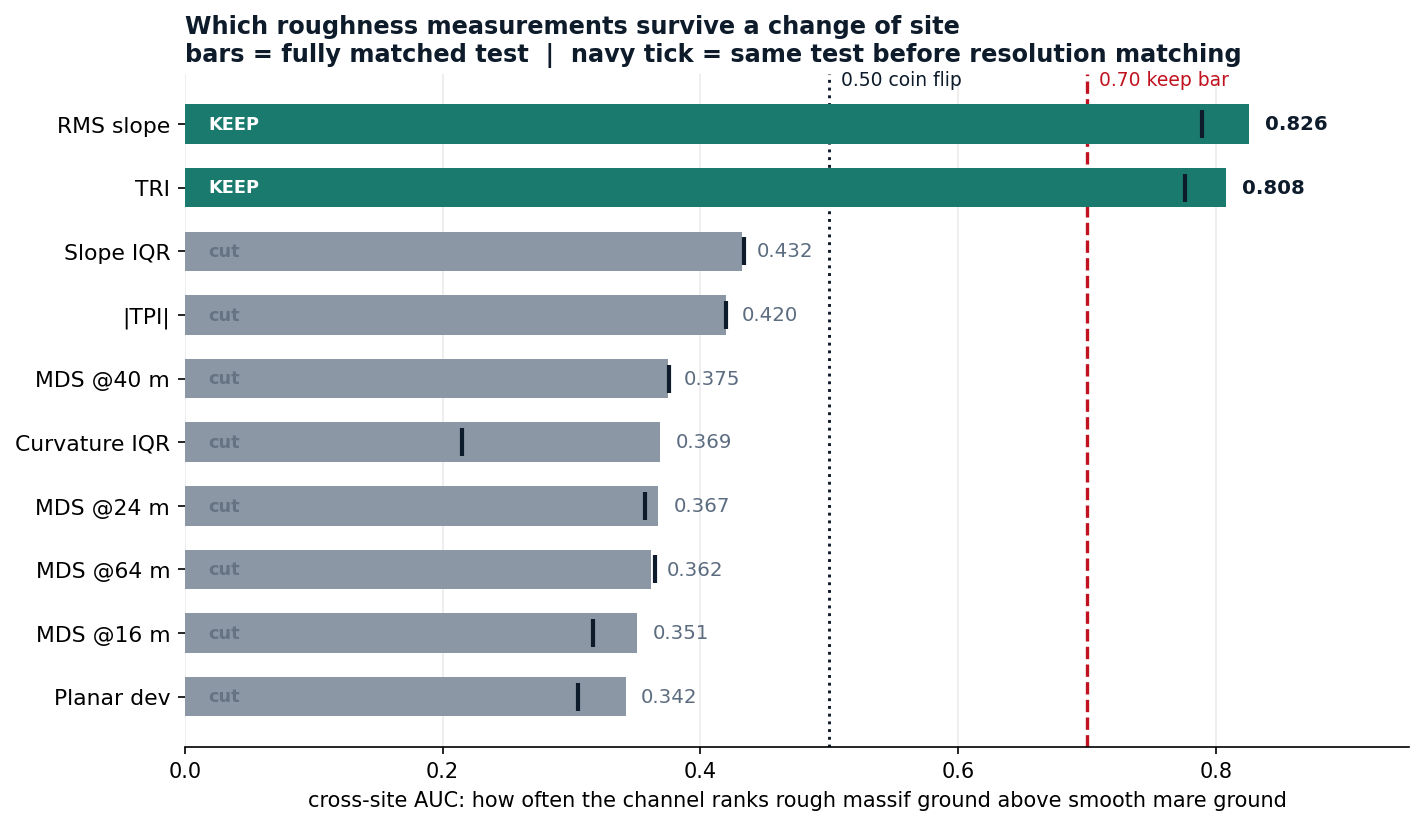
\includegraphics[width=\textwidth]{channel_verdict.png}
\caption{Every roughness measurement HATI originally used, scored on whether it still
works when you move it to a different place on the Moon. Green bars cleared the bar
and were kept. Grey bars were cut. The navy tick marks where each measurement scored
before the test was made fair.}
\label{fig:verdict}
\end{figure}

\subsection{What you are looking at}

HATI originally measured surface roughness ten different ways. Names like ``Slope
IQR'' and ``MDS at \SI{16}{\meter}'' are just different statistical recipes for
``how bumpy is this patch''.

To find out whether those recipes are trustworthy, we ran a controlled test. We took
two places on the Moon we already know the answer for: a smooth lava plain in Mare
Tranquillitatis, near where Apollo 11 landed, and the rough highland massif of Mons
Mouton where Athena came down. A good roughness measurement should score the massif
higher than the plain. Every measurement was scored by how often it does that. That
score is the AUC from the previous section, and it is what the bars show.

Making the comparison fair took care. Both places were first resampled to the same
grid spacing, then blurred so that both carry the same amount of genuine detail. This
second step matters more than it sounds. The Apollo 11 map starts at \SI{2}{\meter}
per pixel and the Mons Mouton map at \SI{4}{\meter}, so without that correction the
smoother site would look artificially more detailed and the test would be rigged.

\subsection{What it means}

Only two measurements cleared the bar.

\begin{center}
\begin{tabular}{lcl}
\toprule
Measurement & AUC & Verdict \\
\midrule
RMS slope & \num{0.826} & Keep. Right about five times in six. \\
TRI (ruggedness) & \num{0.808} & Keep. \\
\midrule
Slope IQR & \num{0.432} & Cut. Below a coin flip. \\
Curvature IQR & \num{0.369} & Cut. Below a coin flip. \\
Planar deviation & \num{0.342} & Cut. \\
$|$TPI$|$ & \num{0.420} & Cut. \\
MDS, all four scales & \num{0.35} to \num{0.38} & Cut. \\
\bottomrule
\end{tabular}
\end{center}

The two that survived have something in common. RMS slope is measured in degrees and
TRI in metres. They are \emph{physical} quantities, and a degree is a degree wherever
you stand. The eight that failed are all measures of \emph{texture}, statistical
descriptions of how varied a patch is, and it turns out those descriptions depend so
heavily on the specific place they were tuned on that they do not survive the move.

One result deserves a direct explanation because it is easy to misread. Curvature IQR
improved a great deal, climbing from \num{0.215} to \num{0.369} once the resolution
mismatch was corrected. That is a genuine improvement of \num{0.153} and it tells us
something real about how much resolution matching matters. But it finished at
\num{0.369}, which is still below \num{0.50}. It got substantially less wrong without
ever becoming useful. Improvement and usefulness are different things, and only the
second one earns a place in the model.

\begin{keepbox}
HATI used to have ten roughness measurements. After this test it has two: RMS slope
and TRI. The other eight were removed. This makes the system simpler and easier to
defend, because every part that remains has evidence behind it.
\end{keepbox}

\begin{limitbox}
This is a negative result about our own work, and it was not the outcome we wanted.
We report it because a measurement that scores below a coin flip on a controlled test
has no business being in a safety system, and because a reviewer would find this in
five minutes if we hid it.
\end{limitbox}

% ---------------------------------------------------------------- fig2
\section{Figure 2: the slope gate, and where Athena falls}

\begin{figure}[h]
\centering
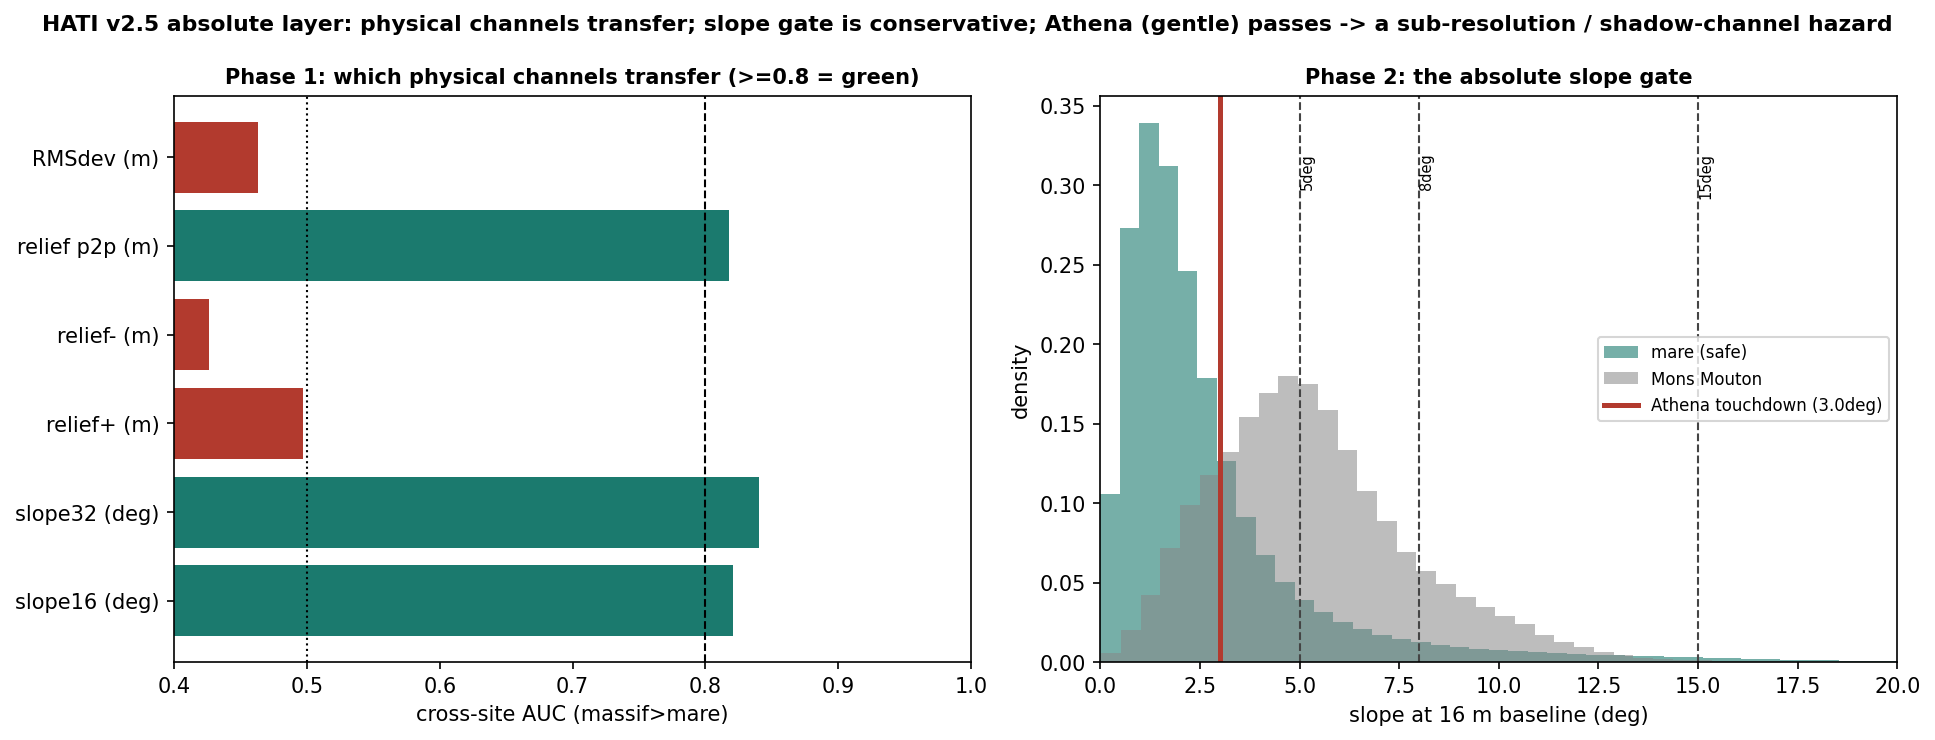
\includegraphics[width=\textwidth]{hati25_absolute_gate.png}
\caption{Left: which measurements transfer between sites, the same test as
\cref{fig:verdict} in its earlier form. Right: how steep the ground is at the two
sites, drawn on one shared scale, with the lander's limit marked and the Athena
landing point shown in red.}
\label{fig:gate}
\end{figure}

\subsection{What you are looking at}

The right-hand panel is the important one. It shows two histograms, which are just
counts of how much ground falls at each steepness. The green shape is the safe lava
plain. The grey shape is the rough massif. The dashed vertical lines mark candidate
lander limits at \ang{5}, \ang{8} and \ang{15}. The red line marks the exact spot
where Athena landed.

\subsection{What it means}

Set the limit at \ang{8}, which is a reasonable value for a lander of this class.
Then:

\begin{itemize}
\item \SI{5.26}{\percent} of the known-safe plain gets flagged. That is the false
alarm rate, and it is an upper bound rather than a true error, because the plain does
contain some real crater walls steeper than \ang{8}.
\item \SI{14}{\percent} of the rough massif gets flagged.
\item The Athena landing point measures \ang{3.0} and \textbf{passes}. The gate says
this ground is fine.
\end{itemize}

That last line looks at first like a failure. It is not. The gate is doing exactly its
job and reporting, correctly, that the ground Athena landed on is not steep. The thing
that tipped the lander was a crater below the resolution of the map the gate reads.
This is the central finding of the whole project: the hazard that destroyed the
mission was invisible to elevation-based methods in principle, not by accident.

For comparison, the older texture-based approach produced a false alarm rate of about
\SI{20}{\percent} on the same safe ground. The physical gate is roughly four times
more specific.

\begin{keepbox}
The slope gate handles big terrain and does it well. It also proves that big terrain
was not what went wrong at Athena. That is what sends the whole project towards
shadows.
\end{keepbox}

% ---------------------------------------------------------------- fig3
\section{Figure 3: two places, one scale}

\begin{figure}[h]
\centering
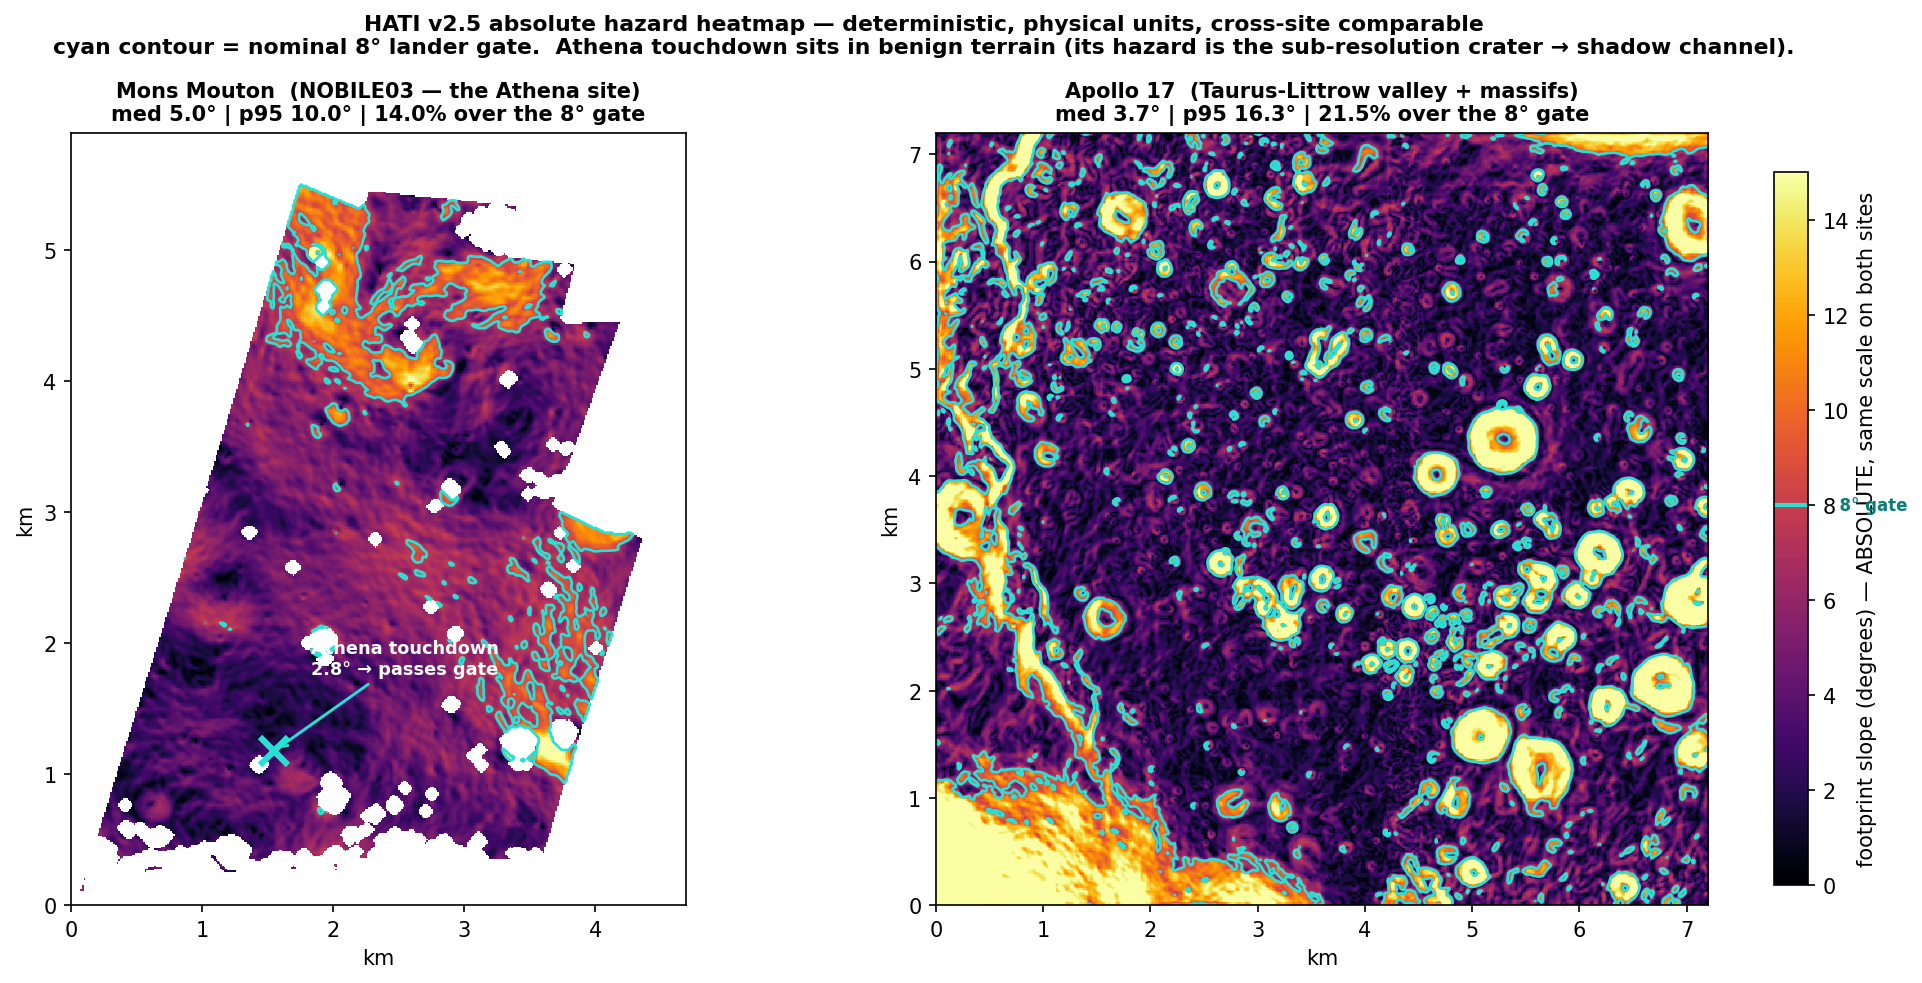
\includegraphics[width=\textwidth]{hati25_heatmaps.png}
\caption{Steepness maps of Mons Mouton, where Athena landed, and the Apollo 17 valley,
drawn with the same colours meaning the same thing on both. The cyan outline traces
the \ang{8} limit. The cross marks the Athena landing point.}
\label{fig:maps}
\end{figure}

\subsection{What you are looking at}

Two maps of different places on the Moon. Dark is flat, bright is steep. Both use the
same colour scale, so a given brightness means the same steepness on both images.

\subsection{What it means}

Being able to put those two maps side by side is the point. Because the measurement is
in degrees, \ang{7} is \ang{7} in both pictures, and you can compare them directly. In
the Apollo 17 panel you can see crater rims and the mountain walls light up, with the
valley floor staying dark, which matches what we know that landscape looks like.

The earlier texture-based approach could not support this comparison at all, because
it scored each scene relative to itself. In that system a value of \num{0.7} meant
``rough compared to whatever else is in this picture'', which is not a measurement of
anything and cannot be carried from one place to another.

% ---------------------------------------------------------------- fig4
\section{Figure 4: using the Sun as a probe}

\begin{figure}[h]
\centering
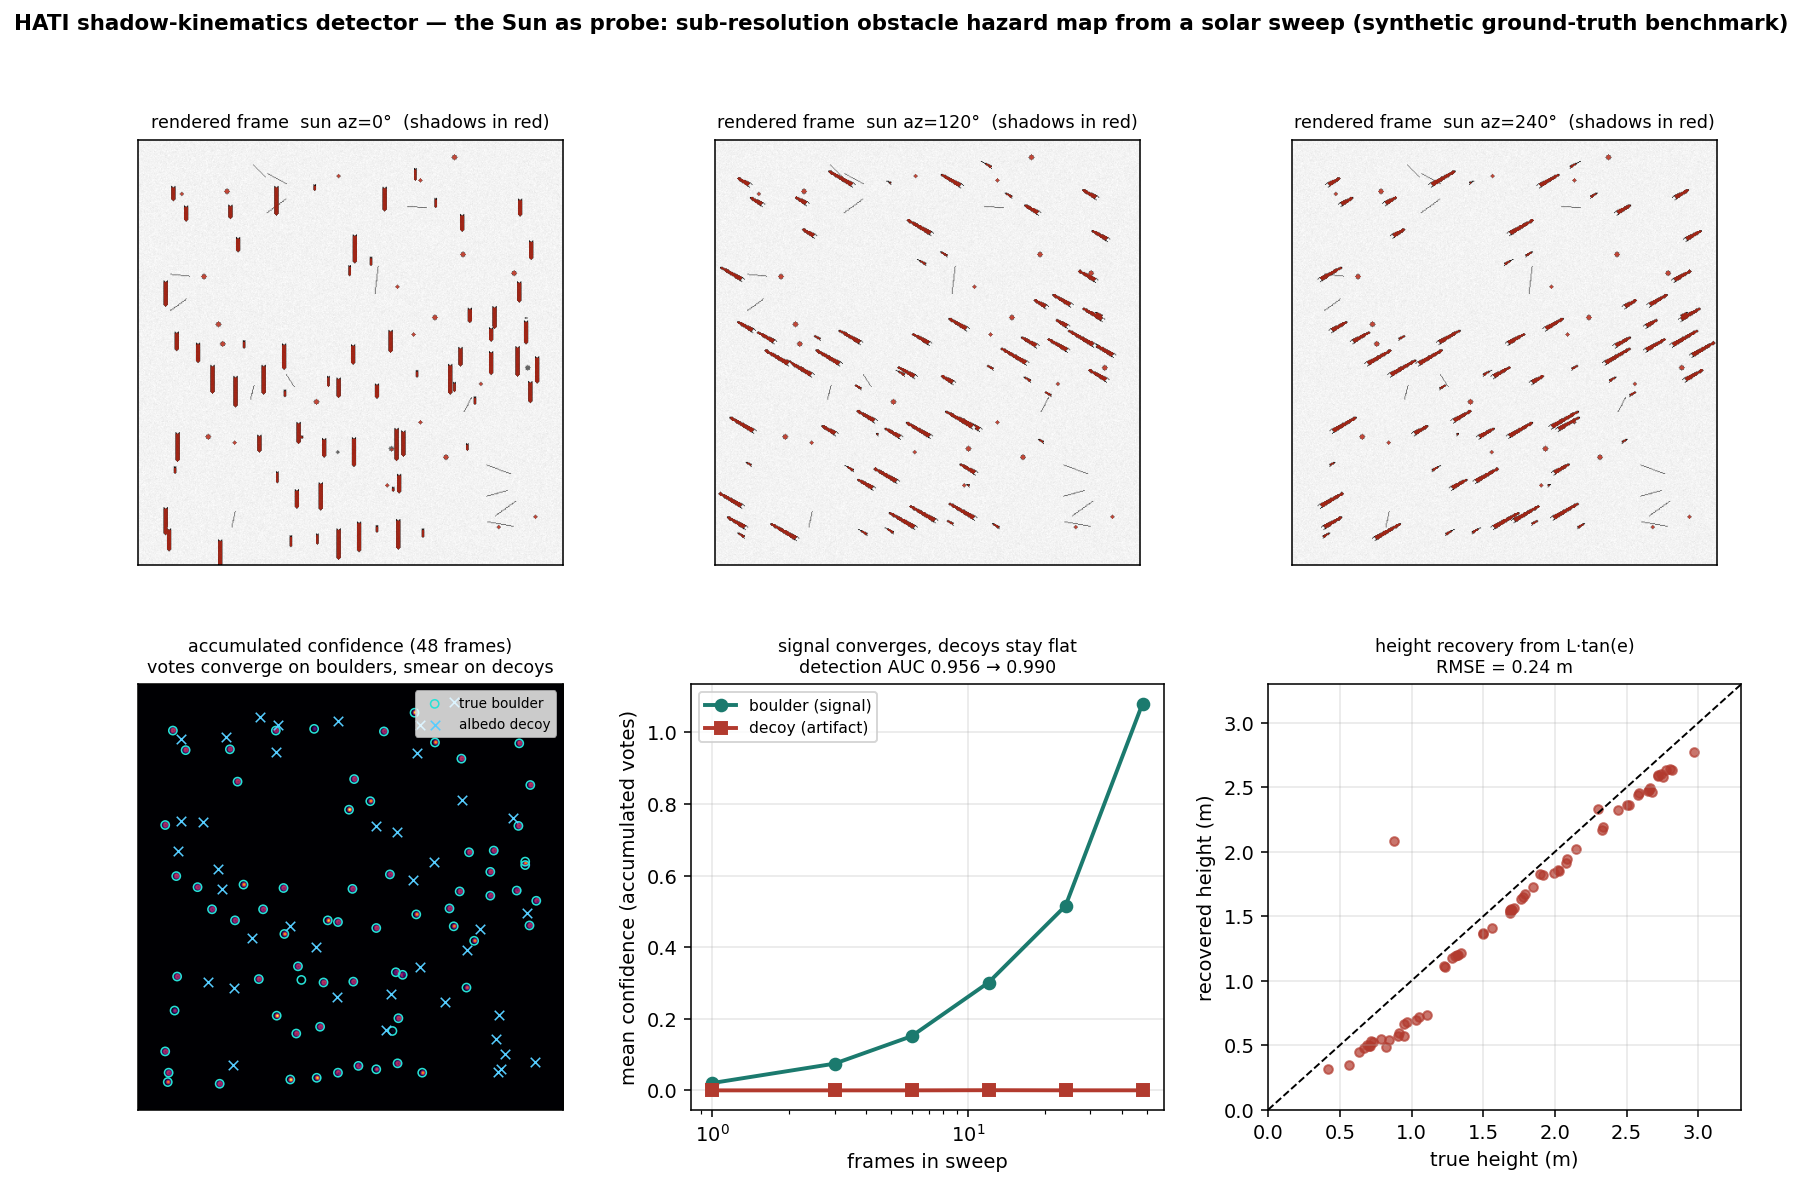
\includegraphics[width=\textwidth]{shadow_kinematics_benchmark.png}
\caption{Top row: the same simulated ground lit from three different Sun directions.
The red shadows swing around their rocks as the Sun moves. Bottom left: accumulated
confidence, bright where the method has decided a real rock stands. Bottom middle:
confidence in real rocks grows with more images while confidence in fake ones stays at
zero. Bottom right: estimated rock heights against their true heights.}
\label{fig:kin}
\end{figure}

\subsection{What you are looking at}

This is the method for finding objects too small for the elevation map, tested on
simulated ground where we planted the rocks ourselves and therefore know every correct
answer.

The scene contains \num{70} rocks between \SI{0.3}{\meter} and \SI{3}{\meter} tall.
All of them are smaller than the elevation map could resolve. It also contains
\num{40} deliberate traps: dark patches and dark streaks that look exactly like
shadows in any single photograph but are simply dark rock.

\subsection{What it means}

The trick is to use the Sun's movement. Over a lunar day the Sun circles the horizon,
so the same ground gets photographed under many different lighting directions. A real
rock's shadow swings around it like the shadow of a sundial gnomon, always anchored at
the rock's base. A dark patch of ground does not move at all, because it is dark for
chemical reasons rather than geometric ones.

So the method drops a vote at the base of every shadow it sees, in every image. Real
rocks collect votes at the same point every time and build up a sharp bright spot.
Fake ones scatter their votes in a ring that never adds up to anything. You can see
exactly this in the bottom middle panel: the green line, which is real rocks, climbs
steadily with more images, while the red line, which is the traps, stays flat on zero.

Once a rock is confirmed, \cref{eq:shadow} converts its shadow length into a height.
The bottom right panel compares those estimates against the truth. The typical error
is \SI{0.24}{\meter}, for rocks between \SI{0.3}{\meter} and \SI{3}{\meter} tall.

\begin{limitbox}
Everything in this figure is simulated. The method works on ground we invented, where
the terrain is flat, the traps come in only two varieties, and the images line up
perfectly. Real images have none of those luxuries. Until this runs on real
photographs, it is a promising estimator and nothing more. The archive check has been
done, so we know the images exist: \num{696} photographs of the Athena site, \num{525}
of them with the Sun up, covering every direction of the compass.
\end{limitbox}

% ---------------------------------------------------------------- claims
\section{What HATI can and cannot say}
\label{sec:cannot}

\begin{center}
\small
\begin{tabular}{p{8.2cm} l p{3.4cm}}
\toprule
Statement & Status & Evidence \\
\midrule
The Athena spot is unusual compared to its surroundings & Established & $z = 3.22$, real data \\
Steepness and ruggedness carry between sites & Established & AUC \num{0.81} to \num{0.83} \\
The slope gate is specific on safe ground & Established & \SI{5.26}{\percent} false alarm \\
Athena's ground was not steep, so the hazard was small-scale & Established & \ang{3.0} measured \\
Texture measurements do not carry between sites & Established, negative & AUC \num{0.34} to \num{0.43} \\
Shadows can separate real rocks from dark patches & Simulated only & Traps score zero \\
Shadows can measure rock height & Simulated only & \SI{0.24}{\meter} typical error \\
The same works on real photographs & Not yet done & Images confirmed to exist \\
A calibrated probability of losing a mission & Not attempted & See below \\
\bottomrule
\end{tabular}
\end{center}

Two limits deserve saying in full.

HATI does not produce a probability that a landing will fail. It produces a hazard
ranking. Turning a ranking into a real probability needs many recorded landing
outcomes to calibrate against, and humanity has only a handful of instrumented lunar
landings. Anyone quoting a percentage chance of failure from this system is
overstating what the data supports.

The $z = 3.22$ figure for the Athena site says that spot is unusual \emph{for that
neighbourhood}. On an absolute scale, measured in degrees and metres, the same ground
is unremarkable. Both statements are true and they are not in conflict, because they
measure different things. The absolute measurement is the one that transfers between
sites, and it is the one to trust for site selection.

% ---------------------------------------------------------------- poseidon
\section{Poseidon: the same idea, at sea}

The interesting thing about the shadow method is that almost nothing in it is about
the Moon. Strip away the setting and what remains is a general recipe:

\begin{quote}
Find objects too small or too faint to see directly, by collecting evidence across
many observations taken under different geometry, where physics predicts how a real
object's signature must change between observations. Reject anything that fails to
change the way physics says it should.
\end{quote}

Project Poseidon applies that recipe to maritime surveillance. The problem there is
dark vessels: ships that switch off their transponders, which is exactly when they
most want watching. Illegal fishing boats do it. Sanctioned tankers do it. So do
vessels loitering above undersea cables and pipelines, which since the Nord Stream
attacks has become a serious concern in the Baltic and North Sea.

\subsection{The physical bridge}

The transfer is closer than it looks, and it is not a loose analogy.

On the Moon, the length of a shadow encodes the height of the rock that cast it, by
\cref{eq:shadow}. At sea, radar satellites have a comparable quirk. In a synthetic
aperture radar image, a moving target is displaced sideways in the picture by an amount
proportional to how fast it is moving towards or away from the satellite:
\begin{equation}
\Delta x \;\approx\; \frac{R}{V}\,v_r
\label{eq:sar}
\end{equation}
where $R$ is the range to the target, $V$ the satellite's speed, and $v_r$ the ship's
speed along the line of sight. A moving ship therefore appears offset from its own
wake, and the size of that offset tells you its velocity.

The shapes of \cref{eq:shadow} and \cref{eq:sar} are the same. One physical property
of an object, recovered from a geometric displacement, using nothing but known
geometry. The auditability that makes HATI defensible carries across unchanged.

\begin{center}
\small
\begin{tabular}{ll}
\toprule
HATI, on the Moon & Poseidon, at sea \\
\midrule
The Sun moves through many angles & The satellite revisits at many angles \\
Shadow length gives rock height & Wake offset gives ship velocity \\
Dark rock that never moves is rejected & Sea clutter that ignores physics is rejected \\
Votes converge at a rock's base & Detections stay consistent across passes \\
Slope gate handles big terrain & Standard clutter filtering handles easy cases \\
Cross-checked against Diviner rock counts & Cross-checked against transponder records \\
\bottomrule
\end{tabular}
\end{center}

\subsection{Why the sea is the easier place to prove it}

There is a real strategic advantage here. HATI has essentially one instrumented
landing to check itself against. Poseidon has transponder data, which is public,
continuous, and covers thousands of ships every week.

That flips the usual relationship. Match a radar detection against the transponder
records and you can measure precisely how often the method is right. And the
detections that have \emph{no} matching transponder record are not errors to be
explained away. They are the product, because a ship the radar sees and the
transponder does not report is exactly the dark vessel a coast guard wants to know
about.

The practical route is short. The European Sentinel-1 satellites provide radar images
of the sea free of charge, day, night and through cloud \autocite{torres2012}. Ship
detection in radar imagery is a mature field with established baselines to measure
against \autocite{crisp2004}. A first test needs one radar scene over a stretch of the
Baltic, the matching transponder records for the same hours, and a comparison of the
two.

\begin{limitbox}
Some things do not carry over, and pretending otherwise would be dishonest. Radar
physics is not shadow physics, so the front end of the detector has to be rebuilt. The
sea surface moves, unlike lunar terrain. Radar images carry speckle, a grainy
interference pattern with statistics quite unlike ordinary image noise. What transfers
is the method and the discipline, not the code.
\end{limitbox}

% ---------------------------------------------------------------- glossary
\section{Glossary}

\begin{description}[leftmargin=!,labelwidth=3.1cm,style=nextline]
\item[AUC] How often a measurement correctly picks the rougher of two random patches.
\num{0.5} is guessing, below \num{0.5} is reliably wrong.
\item[DEM] Digital Elevation Model. A map storing the height of the ground at each pixel.
\item[Effective resolution] The size of the smallest feature a map can genuinely show,
usually several times coarser than its pixel spacing suggests.
\item[False alarm rate] How often a system flags ground that is actually safe.
\item[NAC] Narrow Angle Camera, the high-resolution camera on NASA's Lunar
Reconnaissance Orbiter \autocite{robinson2010}.
\item[Orthophoto] A photograph corrected so that distances in the image match
distances on the ground.
\item[RMS slope] A measure of average steepness across a patch, in degrees.
\item[SAR] Synthetic Aperture Radar. A radar that builds a detailed image using the
satellite's own motion, and works through darkness and cloud.
\item[Solar sweep] A set of photographs of the same place taken under many different
Sun directions.
\item[TRI] Terrain Ruggedness Index. The average height difference between a point and
its immediate neighbours, in metres \autocite{riley1999}.
\item[z-score] How unusual a value is compared to its surroundings, counted in typical
spreads.
\end{description}

% ---------------------------------------------------------------- sources
\section{Sources and further reading}

The roughness measurements HATI started from come from the planetary science
literature, chiefly the work on lunar and martian surface roughness by
\textcite{kreslavsky2000}, \textcite{rosenburg2011} and \textcite{kreslavsky2013}, with
later refinements in \textcite{caifa2020}. The ruggedness index is older and comes from
terrestrial geomorphology \autocite{riley1999}.

The imagery and elevation data are from the Lunar Reconnaissance Orbiter Camera
\autocite{robinson2010}, with the stereo elevation models built by the method of
\textcite{henriksen2017}. Where surface brightness needs a physical model, the standard
reference is \textcite{hapke1984}, with lunar parameters mapped by
\textcite{sato2014}. The limit on what any sampled grid can represent is the classic
sampling result of \textcite{shannon1949}.

For the maritime work, the Sentinel-1 radar mission is described by
\textcite{torres2012} and the state of ship detection in radar imagery by
\textcite{crisp2004}.

\begin{limitbox}[A note on the references]
The two maritime references were recalled from memory rather than looked up, and are
marked as unverified in the bibliography file. Confirm the author lists, volumes and
page numbers before this document is submitted anywhere. The lunar references have been
carried through earlier HATI papers, but a fresh check costs little.
\end{limitbox}

\printbibliography[title={References}]

\end{document}
